\documentclass[a4paper,12pt]{article}
\usepackage[utf8]{inputenc}
\usepackage[brazil]{babel}
\usepackage{booktabs}
\usepackage{caption}
\usepackage[a4paper,top=2cm]{geometry}
\usepackage{graphicx}
\usepackage{amsmath, amssymb, amsthm}
\usepackage{listings}
\usepackage{xcolor} 
\usepackage{enumitem}
\usepackage{csquotes}
\usepackage[backend=biber,style=authoryear]{biblatex}
\usepackage{algorithm}
\usepackage{algorithmic}
\usepackage{booktabs} 
\usepackage{siunitx}  
\usepackage{pgfplots}
\pgfplotsset{compat=1.18}


\addbibresource{referencias.bib}

\lstset{
    basicstyle=\ttfamily\small,
    keywordstyle=\color{blue},
    stringstyle=\color{red},
    commentstyle=\color{gray},
    numbers=left,
    numberstyle=\tiny\color{gray},
    breaklines=true,
    tabsize=4,
    showstringspaces=false,
}


\title{Alocação de Registradores Utilizando Coloração em Grafos}

\author{Raoni Silva, Raul Ramalho}
\date{\today}

\begin{document}

\maketitle

\noindent Turma de Grafos 35M34 \\ Unidade 3

\newpage

\tableofcontents


\section{Resumo}

Investigação do estado da arte sobre otimização do uso de registradores com variáveis pelas técnicas de modelagem com coloração de grafos de interferência. Investigação de sua evolução histórica, mensuração dos resultados e desfecho.
\section{Introdução}

Registradores são componentes de memória de uso genérico de uma CPU de um computador.
Sua função é de armazenar dados e intruções que serão processados de imediato. É a tecnologia de maior nível na hierárquia de memória em um computador.

Pela sua quantidade reduzida, uso intermitente e alta importância, sua ociosidade ou desperdício não é desejável.
O uso ótimo destes componentes é portante prioritário. Para isso, pesquisa e técnicas de otimização foram desenvolvidas nesta área.

Entre as diversas abordagens disponíveis, uma delas adotadas fora a de coloração de grafos de interferência. Técnica que consiste
em cada variável em dado programa de computador é representada por um vértice no grafo, e suas arestas representam a coexistência
do tempo de vida desta variável no mesmo instante. Cada cor atribuída ao grafo corresponde ao número de registradores de propósito geral disponíveis.

Inicialmente, em 1981 nos laboratórios da IBM, o cientista Chaitin e seus colegas de pesquisa desenvolveram o primeiro algoritmo otimização
do uso de registradores com coloração de grafos de interferência.

O algoritmo é especificado em quatro etapas, construção do grafo de interferência, armazenamento na memória e coloração, spilling
( armazenamento na ram) e recuperação das variáveis na ram e recosntrução do grafo.

Posteriormente, o cientista \textcite{briggs} e seus colegas da Rice University, interessados no problema decidem refinar o
algoritmo de \textcite{chaitin} e companhia, resultando na aprimoração das heurísticas na etapa de coalescência, simplificação e spilling(derramamento).

Por fim, em 1996, pelo Bell Labs na equipe de George e Appel et al., novamente, a técnica de coloração de grafos de interferência
fora otimizada mais uma vez apartir de Briggs e companhia. Agora, a técnica de coalescência admite uma nova heurística, critérios
mais robustos foram atribuidas como prevenção do pior caso do algoritmo de seus antecessores. Uma nova etapa de congelamento
fora adiciona antes de ocorrer o spilling. Atingindo, assim, o estado da arte.

\section{Descrição do problema}

O problema de alocação de registradores consiste em atribuir variáveis a um número limitado de registradores durante a compilação de um programa.

\subsection{Objetivo do problema}

O objetivo é estabelecer uma associação entre as variáveis do programa e os registradores disponíveis,
determinando, sempre que possível, a qual registrador cada variável será atribuída.

Uma solução considerada ótima é aquela que utiliza o menor número possível de registradores para
alocar todas as variáveis do programa.

Por exemplo, considere um programa com cinco variáveis. Em uma primeira tentativa de alocação, cada variável é atribuída
a um registrador diferente, totalizando cinco registradores utilizados. Essa é uma solução válida.
No entanto, se for possível alocar todas as cinco variáveis utilizando apenas três registradores,
essa será uma solução melhor. Além disso, se o número disponível de registradores for de fato três,
essa alocação representa uma solução ótima, pois atende à limitação de recursos.

Em certos casos, pode não existir uma solução válida com o número disponível de registradores, ou seja, não é possível
atribuir cada variável a um registrador sem conflitos. Nesses cenários, a literatura propõe abordagens alternativas,
como a técnica de \textit{spilling}, que transfere algumas variáveis da memória rápida (registradores) para
a memória principal (RAM) durante a execução.

\subsection{Entradas esperadas}

A entrada do problema consiste em uma descrição das variáveis do programa e suas interações,
indicando quais variáveis estão ativas ao mesmo tempo e, portanto, não podem compartilhar o mesmo registrador.

Essa descrição pode assumir diferentes formas, como uma tabela de intervalos de uso de variáveis (lifetimes),
uma matriz de interferência, ou qualquer outro formato que permita inferir conflitos de uso simultâneo entre variáveis.

\subsection{Saídas esperadas}

A saída deve indicar se existe uma atribuição válida das variáveis aos registradores disponíveis.
Caso exista, a solução deve apresentar a alocação realizada, especificando a qual registrador cada variável foi atribuída.

Em caso de impossibilidade (isto é, se não for possível realizar a alocação com o número de registradores fornecido),
a saída deve indicar que não há solução válida. Alternativamente, pode apresentar uma solução com \textit{spilling},
identificando quais variáveis foram movidas para a memória.

\section{Modelagem em grafos}

Para a modelagem do problema, considere os vértices como representações das variáveis do programa,
e as arestas indicam conflitos entre variáveis — isto é, situações em que duas variáveis estão ativas
ao mesmo tempo e, portanto, não podem compartilhar o mesmo registrador. O grafo formado por essa relação
é chamado de \textit{grafo de interferência}.

Dessa forma, uma coloração adequada do grafo de interferência — atribuindo uma cor diferente
para cada conjunto de variáveis que não podem ser simultâneas — corresponde a uma alocação de registradores sem conflitos.

Se a coloração do grafo puder ser feita com um número de cores menor ou igual ao número de registradores disponíveis,
então é possível realizar a alocação diretamente. Caso contrário, é necessário utilizar alguma técnica de spilling para
lidar com as variáveis que não puderem ser atribuidas a um registrador.

\section{Estado da Arte}

o estado da arte foi alcançado pelo laboratório bell labs innovations através do algoritmo de  \textcite{irc}.
o algoritmo consiste no aprimoramento dos trabalho de \textcite{briggs} e \textcite{chaitin}.

a diferença mais aguda entre o trabalho de briggs e george e appel foi a introdução de uma etapa de freezing ( congelamento ) antes de spillar ( derramar ) a variável na cpu. esse estado intermediário decidirá quando a variável deve ser reintroduzida no grafo original ou se será armazenada à ram.

também fora incrementado a heurística de coalescência, tornando-o mais agressiva com a regras de briggs permitindo uma maior eficácia na fusão de variáveis. 



\section{Descrição do Algoritmo}

O algoritmo de George-Appel funciona através da construção de um grafo de interferência iterativo, e posteriormente, K-colorido, onde K é o número de registradores. Ao todo, possui sete etapas.\textit{ build, simplify, conservative coalesce, freeze, potential spill, select e actual spill}. Adota o estilo de Coalescência Conservadora de Briggs e a simplificação de Chaitin resultando em uma maior eficiência que ambas as técnicas separadas. A nova abordagem para alocação de registradores com grafos de interferência iterativo garante uma execução em loop das etapas, retomando, em laço, as etapas de simplficação, coalescência, congelamento e derramamento inúmeras vezes no mesmo grafo. Tal característica torna dificil estimar a complexidade do algoritmo.



\textit{Build:} Constrói o grafo de interferência e categoriza os vértices entre instruções de cópia (move related) ou não.


\textit{Simplify:}  Remove as instruções de cópia de menor grau no grafo.


\textit{Conservative Coalesce:} Atua semelhante ao algoritmo de Briggs.

\textit{Freeze: } Nem simplifica nem coalesce, busca instruções cópia de baixo grau e as congela. Retorna às etapas de simplificação e coalescência

\textit{Select: } Mesma etapa dos algoritmos anteriores, exceto que não adotada bias na hora do julgamento para otimização precoce de instrução de moves.

\textit{Spill: } Armazena as variáveis na memória RAM para retorná-las futuramente.

Uma instrução de cópia ( ou move instruction ) é quando uma variável está armazenada no registrador temporário de origem e passa ao registrador de destino ( onde será processada ).

\subsection{Pseudocódigo e Complexidade: }

Dado os retornos sucessivos à etapa de build, e as sucessivas iterações e interoperações entre etapas de congelamento, derramento, coalescência, simplificação e seleção. É de enorme dificuldade estimar a complexidade global do algoritmo.

O pseudocódigo utilizado fora o original do artigo de George-Appel et al, 1996, página 19 à 23.

\begin{center}
    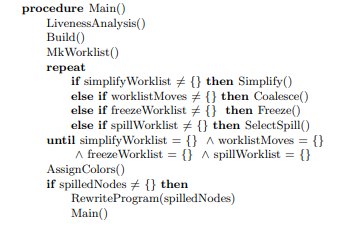
\includegraphics[scale=0.6]{img/code1.png}
    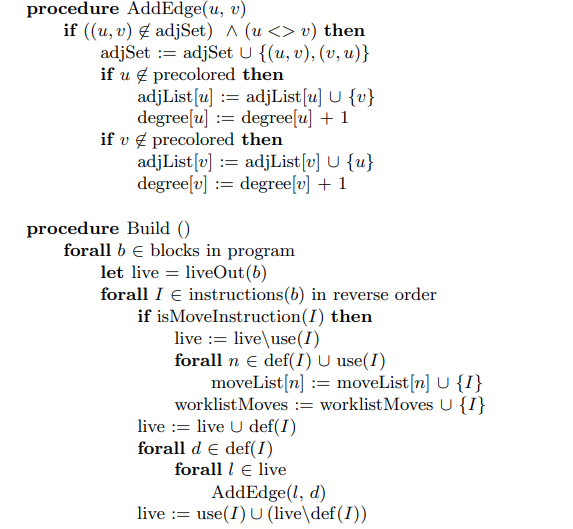
\includegraphics[scale=0.6]{img/code2.png}
    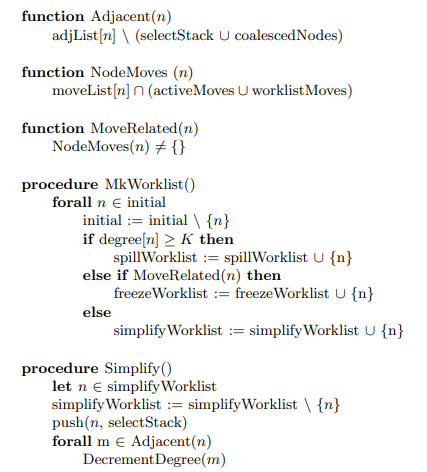
\includegraphics[scale=0.6]{img/code3.png}
    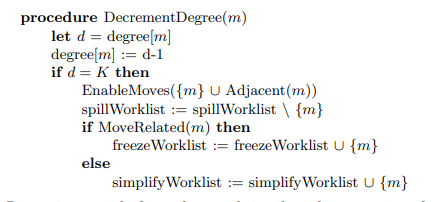
\includegraphics[scale=0.6]{img/code4.png}
    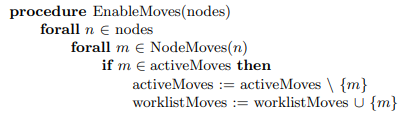
\includegraphics[scale=0.6]{img/code5.png}
    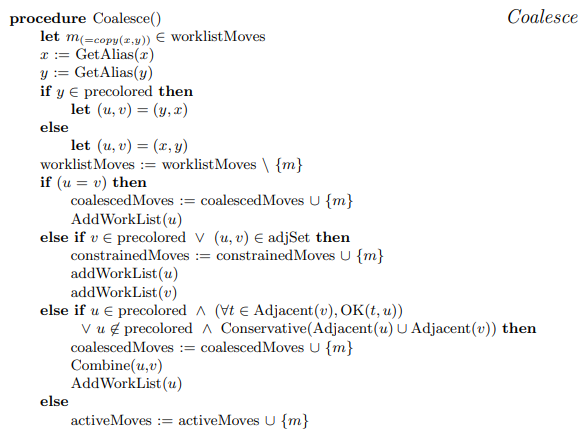
\includegraphics[scale=0.6]{img/code6.png}
    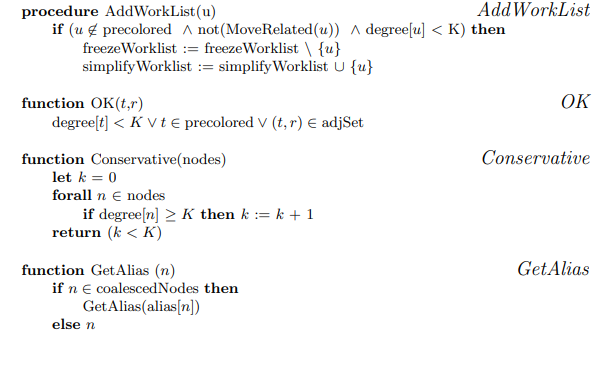
\includegraphics[scale=0.6]{img/code7.png}
    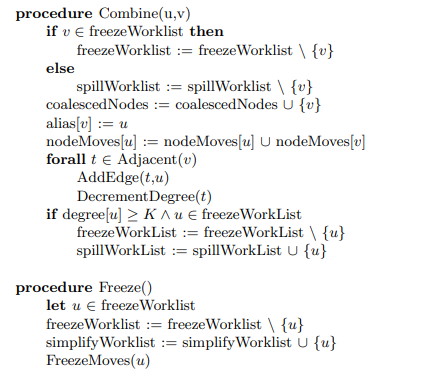
\includegraphics[scale=0.6]{img/code8.png}
    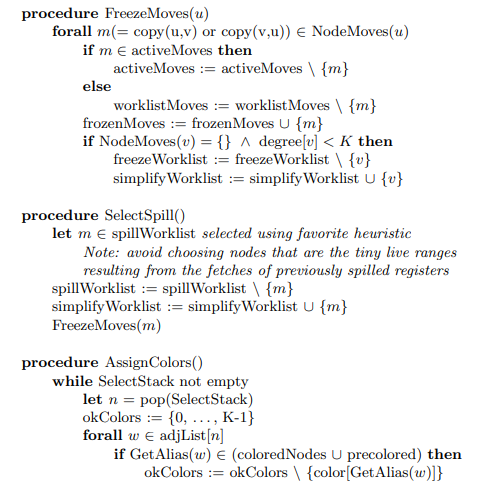
\includegraphics[scale=0.6]{img/code9.png}
    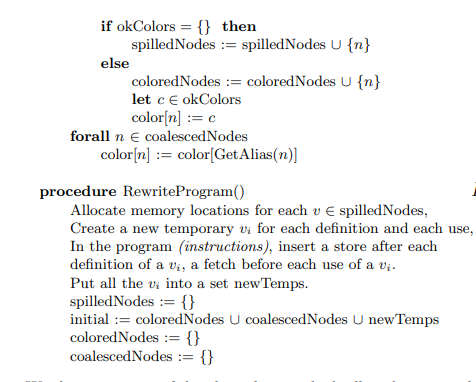
\includegraphics[scale=0.6]{img/code10.png}

\end{center}

Assume-se, que a instânciação do pseudocódigo ao algoritmo em uma linguagem de programação qualquer o implementador usará estruturas de dados eficientes para tal.

Seja A o número de arestas de interferência, V o número de vértices, K o número de registradores e M o número de instruções.

\textit{addEdge:} Abrevia-se a complexidade dessa instrução para $O(1)$.

\textit{Build:} Rotina responsável por criar os vértices e arestas, logo $O(V + A)$.

\textit{MkWorklist: } Itera até $n$ vezes o tamanho de $initial$, logo $O(n)$.

\textit{Simplify: } Dado um nó $n$, itera sobre seus vizinhos $adj(n)$, o que custa $O(d(n))$.

\textit{DecrementDegree: } Poucas comparações, justificamente análoga à addEdge.

\textit{EnableMoves: } Itera sobre os nós e a lista de instruções. Custo total $O(V + M)$.

\textit{Coalesce: } O custo de coalesce depende da complexidade dos vértices vizinhos chamados para a coalescência, logo $O(adj(u) + adj(v))$.

\textit{Combine: } Itera sobre todos os vertices pertencentes à adjacente, logo $O(d(vertice))$.

\textit{Freeze: } Custo $O(1)$ pois evoca FreezeMoves.

\textit{FreezeMoves: } Custo $O(M)$ pois itera o vetor do número de instruções.

\textit{SelectSpill: } Depende diretamente de quanto derramamento será causado no programa, pode ser $O(1)$ ou $O(V)$.

\textit{AssignColors: } Irá atribuir cores a todos vértices, logo $O(V)$.


A soma das complexidades individuais não representa a complexidade global do algoritmo, dado que o processo iterativo ocorre inúmeras vezes e chamadas de congelamento, derramamento, simplificação ocorrem inúmeras vezes no mesmo código.

\section{Descrição dos Experimentos Computacionais}

\subsection{Metodologia de testes}

Os experimentos foram feitos a partir de um gerador customizado de instâncias de testes, onde 
é possível simular programas da forma mais fiel possível. Foram gerados 15 instâncias de programas 
com características variadas, e o algoritmo de George-Appel foi executado 3 vezes para cada instância.
Por meio dessa base de dados é possível obter métricas sobre os resultados obtidos, tais como:


\begin{description}
  \item[Tempo de execução:] Medido em milissegundos, representa o tempo de cada execução individual da heuristica com uma certa entrada de dados.
  \item[Quantidade de variáveis:] Representa a quantidade total de variáveis ao final do processo de iterativamente simplificar, coaslescer os nós 
    e reescrever o código.
  \item[Quantidade de variáveis despejadas:] Ao fim da quarta execução, na nossa implementação o algoritmo desiste de encontrar uma solução melhor que reduza a 
    quantidade de nós despejados e finaliza sua execução.
\end{description}


\subsubsection{Simulador de programas}

Para conseguir entradas válidas para o algoritmo, é necessário prover de antemão quais são as variáveis, em que linhas as variáveis são utilizadas e também,
quais são os nós provenientes de operações de moves. Para isso, foi construido um simulador simplificado de programas, ele recebe como entrada parâmetros tais como:


\begin{description}
  \item[ID:] Um identificador para salvar em um arquivo os dados simulados.
  \item[Número de variáveis:] Quantidade de variáveis que serão simuladas no programa.
  \item[Quantidade de moves:] Quantidade de arestas que serão criadas como operações de moves, essas arestas são especiais pois, na prática, significa que o início 
    da vida de uma das variáveis é exatamente no final da vida da outra variável, em uma operação do tipo (x = y). Dessa forma, essa informação deve ser considerada
    ao gerar a lista de linhas de usos de cada variável.
  \item[Limite inferior:] Menor quantidade de linhas de código em que a variável é utilizada.
  \item[Limite superior:] Maior quantidade de linhas de código em que a variável é utilizada.
  \item[Linhas de código:] Quantidade de linhas de código totais no código.
\end{description}

Com isso, foram gerados casos de teste variando principalmente o 
número de variáveis: 10, 100, 200, 500 e 1000. E o limite superior de usos de variável: 5, 15, 30. 
Com cada combinação desses valores sendo uma instância de entrada de dados para o algoritmo. Além disso, foram alteradas a quantidade de moves, mas os resultados
não melhoraram ou pioraram. Além disso, como padrão, foi utilizado 32 como a quantidade de registradores disponíveis para coloração.

\subsubsection{Plataforma de execução}

Todas as execuções foram realizadas em uma única máquina para melhorar a consistência dos dados obtidos. A configuração do ambiente foi:

\begin{itemize}
  \item Hardware:
    \begin{description}
      \item[CPU:] Ryzen 5 5600
      \item[RAM:] 16GB DDR4 2400Mhz
    \end{description}
  \item Software:
    \begin{description}
      \item[Sistema Operacional:] Fedora 41
      \item[Linguagem:] Python 3.13
      \item[Project Manager:] UV(\textcite{uv})
    \end{description}
\end{itemize}


\subsection{Como reproduzir os testes}

Para a reprodução dos experimentos, recomenda-se o uso da ferramenta de gerenciamento 
de pacotes \textbf{UV} (\textcite{uv}) para a criação de um ambiente Python consistente.

O processo consiste em dois passos principais:

\begin{enumerate}
    \item \textbf{Gerar as instâncias de entrada:} Execute o comando abaixo no terminal 
    para criar os cinco arquivos de teste que servirão de entrada para o algoritmo.
    
    \begin{center}
        \texttt{uv run src/generator.py}
    \end{center}

    \item \textbf{Executar o algoritmo:} Após a geração das instâncias, utilize o 
    seguinte comando para executar o algoritmo de coloração de grafos sobre os 
    cinco arquivos gerados.
    
    \begin{center}
        \texttt{uv run src/george-appel.py}
    \end{center}
\end{enumerate}


\section{Resultados Obtidos}

A execução dos experimentos em um conjunto de instâncias variadas permitiu uma análise aprofundada do comportamento da heurística de alocação de registradores.
Os testes foram projetados para avaliar o desempenho do algoritmo sob diferentes cenários de pressão de quantidade de usos de cada variável
(variando o limite superior) e a quantidade de variáveis. A seguir, são apresentados e discutidos os resultados quantitativos.

\subsection{Resultados Quantitativos}

Os experimentos foram executados três vezes para cada configuração, e os tempos de execução foram registrados.
A Tabela~\ref{tab:resultados} consolida estes dados, apresentando o tempo médio de execução e o desvio padrão correspondente para
cada classe de teste e tamanho de instância (número de variáveis).

\begin{table}[h!]
\centering
\caption{Tempo médio de execução e desvio padrão para diferentes cenários de teste.}
\label{tab:resultados}
\sisetup{
  table-format=2.6,
  round-mode=places,
  round-precision=6
}
\begin{tabular}{l l l S}
\toprule
\textbf{Tipo de Teste} & {\textbf{Instância}} & {\textbf{Tempo Médio (s)}} & {\textbf{Desvio Padrão (s)}} \\
\midrule
teste-lim-sup-5   & 10   & 0.000135 & 0.000006 \\
                  & 100  & 0.022424 & 0.000096 \\
                  & 200  & 0.095923 & 0.007000 \\
                  & 500  & 0.654350 & 0.004085 \\
                  & 1000 & 3.753158 & 0.081135 \\
\midrule
teste-padrao      & 10   & 0.000135 & 0.000005 \\
                  & 100  & 0.095402 & 0.001427 \\
                  & 200  & 0.573312 & 0.002754 \\
                  & 500  & 3.807789 & 0.014870 \\
                  & 1000 & 21.030808 & 0.207316 \\
\midrule
teste-lim-sup-30  & 10   & 0.000166 & 0.000043 \\
                  & 100  & 0.328989 & 0.011429 \\
                  & 200  & 1.377198 & 0.029020 \\
                  & 500  & 17.993473 & 0.191330 \\
                  & 1000 & 51.772303 & 0.286317 \\
\bottomrule
\end{tabular}
\end{table}

\subsection{Análise dos Resultados}

A análise dos dados apresentados na Tabela~\ref{tab:resultados} revela tendências importantes sobre o comportamento do algoritmo.

\paragraph{Análise de Escalabilidade} Para todos os tipos de teste, observa-se um crescimento consistente no tempo de execução à medida que 
o número de variáveis da instância aumenta. Este crescimento é notavelmente não linear, indicando que a complexidade do problema de coloração
aumenta significativamente com o tamanho do grafo de interferência. Mesmo com a heurística tendo uma complexidade polinomial, o maior impacto no tempo
de execução se dá por causa da reescrita do "programa". Pois isso adiciona uma quantidade imensa de nós para cada reescrita. Para fins de comparação, observou-se
um aumento na quantidade de nós em alguma execuções com inicialmente 1000 variáveis, terminando com cerca de 8000 variáveis, devido ao split das variáveis que seriam
despejadas.


\paragraph{Impacto da quantidade de usos de variáveis (Limite Superior)} A variação no limite superior de usos de variáveis apresentou o impacto
mais significativo no desempenho.
\begin{itemize}
    \item \textbf{Cenário Intenso (Limite=30):} O teste \texttt{teste-lim-sup-30} foi, de longe, o que apresentou os maiores tempos de execução. Com um grande número de usos de cada variável, a liveness analysis gera intervalos cada vez maiores e com cada vez mais interferências. Além disso, quando as variáveis são divididas em variáveis com tempos de vida menor, a quantidade de variáveis aumenta muito, de forma que a próxima iteração do algoritmo com as novas variáveis demore ainda mais.
    \item \textbf{Cenário Restrito (Limite=5):} Inversamente, o teste \texttt{teste-lim-sup-5} foi o mais rápido. Como existiam menos usos de cada variável, duas coisas importantes acontecem, o liveness dela tende a ser menor, e principalmente, quando ela é dividida em outras variáveis temporárias, a quantidade de variáveis para a próxima execução do algoritmo não aumenta tanto assim, melhorando a eficiência do algoritmo.
    \item \textbf{Cenário Padrão (Limite=15):} O teste \texttt{teste-padrao}, que representa nosso caso base, situa-se entre os dois extremos, indicando um equilíbrio entre as quantidades de variáveis sendo divididas para as execuções seguintes.
\end{itemize}

\subsection{Visualização Gráfica}

Para melhor ilustrar as tendências de escalabilidade e o impacto dos parâmetros, o Gráfico~\ref{fig:grafico-resultados} plota o
tempo médio de execução em função do número de variáveis da instância para cada tipo de teste. A escala do eixo Y é logarítmica
para acomodar a grande variação nos tempos de execução.

\begin{figure}[ht!]
    \centering
    \begin{tikzpicture}
        \begin{axis}[
            title={Desempenho do Algoritmo por Tipo de Teste},
            xlabel={Número de Variáveis (Instância)},
            ylabel={Tempo Médio (s) [escala log]},
            legend pos=north west,
            grid=major,
            width=\textwidth,
            height=8cm,
        ]
        
        \addplot[mark=square*, red] coordinates {(10,0.000166) (100,0.328989) (200,1.377198) (500,17.993473) (1000,51.772303)};
        \addlegendentry{Limite=30}
        
        \addplot[mark=triangle*, green] coordinates {(10,0.000135) (100,0.022424) (200,0.095923) (500,0.654350) (1000,3.753158)};
        \addlegendentry{Limite=5}
        
        \addplot[mark=*, thick, blue] coordinates {(10,0.000135) (100,0.095402) (200,0.573312) (500,3.807789) (1000,21.030808)};
        \addlegendentry{Padrão (Limite=15)}
        
        \end{axis}
    \end{tikzpicture}
    \caption{Comparação do tempo de execução.}
    \label{fig:grafico-resultados}
\end{figure}

O gráfico evidencia claramente o comportamento discutido: a linha correspondente a \texttt{Limite=30} (vermelha) se destaca com os maiores
tempos, enquanto a linha para \texttt{Limite=5} (verde) permanece consistentemente como a mais rápida para instâncias maiores. As demais configurações
apresentam um desempenho intermediário e muito próximo entre si.


\subsection{Discussão sobre a Validade das Instâncias}

Uma consideração fundamental para a interpretação dos resultados é a natureza das instâncias geradas pelo simulador. Especificamente, a implementação atual não modela o \textbf{princípio da localidade}, um comportamento prevalente em software real.

No simulador, os usos de uma variável são distribuídos de forma semi-aleatória ao longo de todo o código. Este método pode gerar variáveis com \textit{live ranges} longos e fragmentados, que se estendem por múltiplos escopos. Tal comportamento contrasta com o de programas típicos, onde o tempo de vida de uma variável é frequentemente restrito a uma única função ou a um laço de repetição.

Como consequência, os grafos de interferência gerados, embora válidos, podem apresentar uma topologia menos comum em cenários práticos. Portanto, os resultados obtidos são uma excelente avaliação da robustez da heurística em grafos complexos, mas a sua performance em códigos com alta localidade não foi avaliada devido a limitação da atual implementação do gerador.

\section{Conclusão}

Neste trabalho, investigou-se a alocação de registradores via coloração de grafos, comparando
implementações dos algoritmos de \textcite{chaitin}, \textcite{briggs} e \textcite{irc}.  
Observou-se que Chaitin apresenta implementação mais simples, mas tende a maior número
de spills em relação a abordagens refinadas.  
Briggs introduz heurísticas de coalescing otimista que reduzem moves, porém aumentam
a complexidade de análise.  
George-Appel (Iterated Register Coalescing) demonstrou maior taxa de coalescência e menos spills,
sendo uma melhoria direta em relação do de Briggs.  
Em suma, refinamentos em coalescing e heurísticas de spill podem melhorar significativamente a geração de código
sem comprometer o tempo de compilação.

\printbibliography





\end{document}
